% Origen: Secciones/PI - Implementacion OSC.md
% El "Apéndice" de la nota va en apend6.tex (Detalles del osciloscopio).
\chapter{Implementación del OSC}
\label{C:osc}

% Figuras de ESTE capítulo + las compartidas. Siempre al principio del archivo.
\graphicspath{{figs/cap8/}{figs/comunes/}}

\begin{destacado}
En este capítulo se describe (1) las funcionalidades que provee el módulo
osciloscopio empleado, (2) el módulo base de Pitaya, con una descripción
detallada del mecanismo de transferencia de datos al PS, sus limitaciones y el
método de utilización de este módulo desde el PS, y (3) una mejora implementada
en el mecanismo de transferencia y su método de utilización desde el PS. Las
figuras de mérito y comparaciones con el sistema original se presentan en la
Sec.~\ref{S:res-throughput-osc}.
\end{destacado}

%==============================================================================
\section{Función del osciloscopio}
\label{S:osc-funcion}

Su nombre deriva de su funcionamiento principal, que es exactamente igual al de
un osciloscopio. El mismo guarda en un buffer interno una \textbf{traza} de la
señal a su entrada. Esta traza consiste en medidas previas y posteriores al
disparador. Este tipo de funcionalidad es típica de un sistema de HW
programable, debido a que es de las mejores formas de debug de un datapath.
Otros puntos importantes de funcionalidad consisten en:
\begin{itemize}
  \item Largo de traza: en la versión base es un buffer circular fijo de
    $2^\text{RSZ}$ muestras por canal (16384 en el diseño original de Pitaya,
    8192 en este proyecto), del que se configura el largo post-trigger; en la
    versión con anillo de eventos (Sec.~\ref{S:osc-anillo-eventos}) la ventana
    \codigo{pre+post} es configurable hasta 1024 muestras (con \codigo{pre}
    $\leq$ 1023), y por defecto vale 32 (\codigo{pre=8}, \codigo{post=24}).
  \item Mediciones a tiempo de clock de sistema o con un diezmado programable
    (desde 1 hasta 65536).
  \item Disparo por una señal de evento (trigger).
\end{itemize}
Como tenemos toda la información del pulso, no consideramos necesario realizar
un procesamiento en HW de seguimiento de línea de base o compensación de la
misma.

\subsection{Caminos de datos}
\label{S:osc-caminos}

La versión original del osciloscopio proveniente de Pitaya implementa
\textbf{dos metodologías de acceso}. Esto puede comprobarse en la
Fig.~\ref{f:osc-panorama-pitaya}, en la que se presentan dos interfaces AXI: la
primera interactúa con AXI\_GP0 mediante el bus interno del sistema
(\codigo{sys\_bus}), mientras que la segunda escribe en la DDR por los puertos
AXI\_HP0 y AXI\_HP1 (mediante dos bridges, ver la
Sec.~\ref{S:top-vista-general}). Esta interfaz utiliza un esquema de volcado de
datos del tipo \emph{fire and forget} hacia una región de memoria DDR; el
problema de este esquema es que no nos dice nada de la segmentación de los
eventos ni de la consistencia en la lectura de los datos. Estos detalles se
presentan en la Sec.~\ref{S:osc-anillo-eventos}.

Mientras que el bus custom utiliza un handshake completo para leer/escribir
secciones de 32 bits (ver la Sec.~\ref{S:intro-hw-bus-custom}). En la
Sec.~\ref{S:osc-flujo-basico} presentamos los detalles de utilización de esta
modalidad.

\subsection{Vista general del osciloscopio base}
\label{S:osc-vista-general}

Un esquema del funcionamiento del mismo se encuentra en la
Fig.~\ref{f:osc-panorama-pitaya}. Vemos dos regiones: \textbf{una sección
compartida} por todos los canales, representada por bloques en gris, y
\textbf{una cadena de adquisición por stream de datos}. A esta última sección la
subdividimos en otras 4; si hacemos una descripción breve individual por módulo
obtenemos:
\begin{itemize}
  \item \textbf{Cadena de acondicionamiento} (bloques azul claro):
  \begin{itemize}
    \item \codigo{rp\_scope\_calib}: calibración de offset y ganancia,
      $y = \mathrm{sat}\big((x + \text{offset}) \cdot \text{gain}\big)$, con
      saturación al rango de la muestra.
    \item \codigo{osc\_filter}: es un ecualizador IIR que tiene como objetivo
      compensar la respuesta en frecuencia del \emph{front-end} analógico
      (coeficientes \codigo{aa/bb/kk/pp} por canal). Estos son los
      coeficientes comentados en la sección de calibración de Pitaya
      (Sec.~\ref{S:hw-calibracion}).
    \item \codigo{rp\_decim}: reduce la tasa de muestreo por un factor de 1 a
      65536, quedándose con una muestra de cada N o promediándolas
      (\codigo{AVG\_EN}). Llamamos a la unidad de tiempo reducida \emph{tick} y
      no \emph{clock}, para no confundirnos con el reloj del sistema.
    \item \codigo{rp\_delay}: como la salida del trigger está desfasada de los
      datos, este módulo lo compensa: 1 ciclo para los triggers por nivel de
      los canales y 2 para el externo y el del ASG.
  \end{itemize}
  \item \textbf{Cadena de triggering} (bloques amarillos): se calcula en
    paralelo a la cadena de acondicionamiento.
  \begin{itemize}
    \item \codigo{rp\_adc\_trig}: utiliza un disparador con histéresis de tipo
      Schmitt sobre el stream \emph{sin retrasar} del diezmador. Emite un pulso
      de un ciclo en cada flanco de subida (\codigo{trig\_p}) y de bajada
      (\codigo{trig\_n}).
    \item \codigo{rp\_trig\_src}: elige una fuente entre los flancos de los
      canales, el trigger externo, el ASG y el de software (código de 4 bits).
  \end{itemize}
  \item \textbf{Manejo de captura}:
  \begin{itemize}
    \item \codigo{rp\_bram\_sm}: implementa la FSM de armado, post-trigger y
      congelado del buffer, sobre la que el PS hace los 3 pasos de la sección
      siguiente. Se explica en detalle en la Sec.~\ref{S:ap-osc-fsm-bram} del
      Apéndice.
  \end{itemize}
  \item \textbf{Manejo de transacciones}:
  \begin{itemize}
    \item \codigo{rp\_acq\_bram}: buffer circular de $2^\text{RSZ}$ muestras de
      14 bits (RSZ = 14 en el original, 13 en este proyecto). Se lee mediante
      el \codigo{sys\_bus}, una muestra por transacción.
    \item \codigo{rp\_axi\_sm}: camino paralelo que hace uso de \emph{direct
      memory access} (DMA). Se describe en detalle en la
      Sec.~\ref{S:osc-anillo-eventos}.
  \end{itemize}
\end{itemize}

\begin{figure}[H]
\centering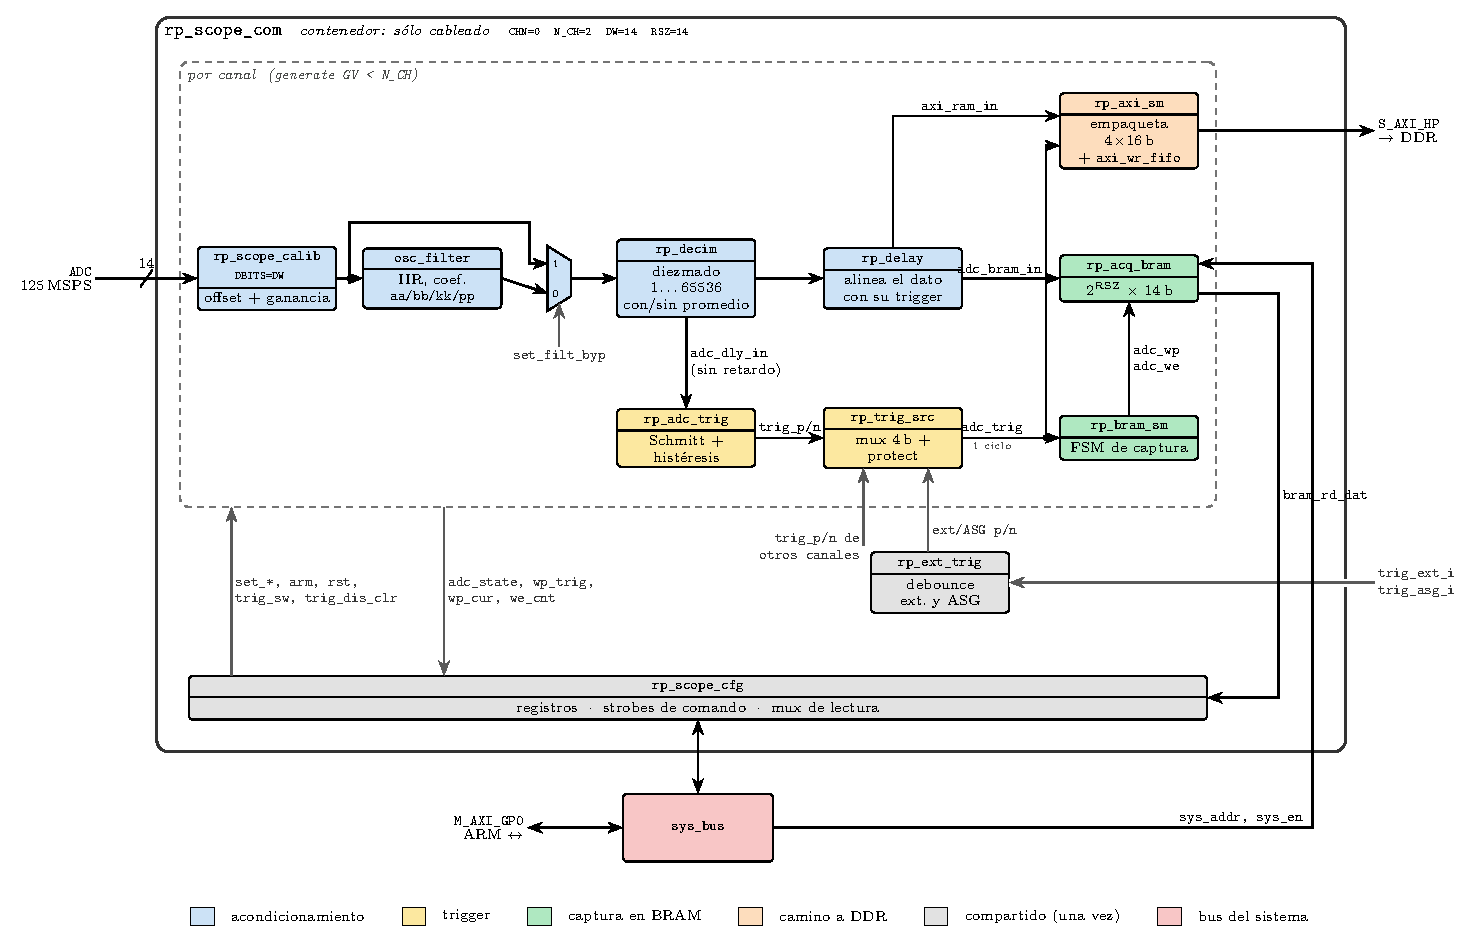
\includegraphics{cap8_panorama_scope_pitaya}
\caption[Módulo OSC original de Pitaya]{%
Módulo OSC original de Pitaya. Contiene una cadena de preprocesamiento (azul),
sección de triggering interno (amarillo) y externo (módulo
\codigo{rp\_ext\_trig} en gris), submódulo de configuración (en gris), lógica de
captura de datos y manejo de transacciones por bus custom (verde) y camino de
datos por HP (\codigo{rp\_axi\_sm} en naranja claro).\label{f:osc-panorama-pitaya}}
\end{figure}

Mientras que si desarrollamos los \textbf{bloques compartidos} encontramos los
dos siguientes:
\begin{itemize}
  \item \codigo{rp\_ext\_trig}: es un \emph{debouncer} de longitud configurable
    para el trigger externo y del ASG.
  \item \codigo{rp\_scope\_cfg}: guarda la configuración y maneja los comandos
    desde SW a la FSM. Multiplexa hacia \codigo{sys\_bus} la lectura del estado
    y de la BRAM.
\end{itemize}

\subsection{Flujo de funcionamiento básico}
\label{S:osc-flujo-basico}

El proyecto base de Pitaya ya contaba con un módulo capaz de implementar una
versión básica de esta funcionalidad mediante el bus custom. En la
Fig.~\ref{f:osc-secuencia-basica} se presentan los pasos para realizar una
captura: primeramente tenemos que realizar todas las configuraciones
necesarias, mientras que por traza capturada tenemos que seguir los siguientes
pasos:
\begin{enumerate}
  \item \textbf{Armado} (\emph{arm}): es mandar el comando de armado
    \codigo{CMD\_ARM}, que se realiza escribiendo un 1 a este registro. Indica al
    módulo que terminó de trabajar con su buffer interno y que es capaz de
    sobreescribirlo.
  \item \textbf{Chequeo de finalización de captura} (congelamiento): se lee la
    variable \codigo{ADC\_STATE} hasta que la vemos en alto. Representa que el
    módulo terminó de adquirir la traza deseada y se encuentra disponible para
    leer.
  \item \textbf{Lectura}: el buffer interno se encuentra congelado; en este
    estado se realizan las transacciones de lectura necesarias para extraer
\end{enumerate}

\begin{figure}[H]
\centering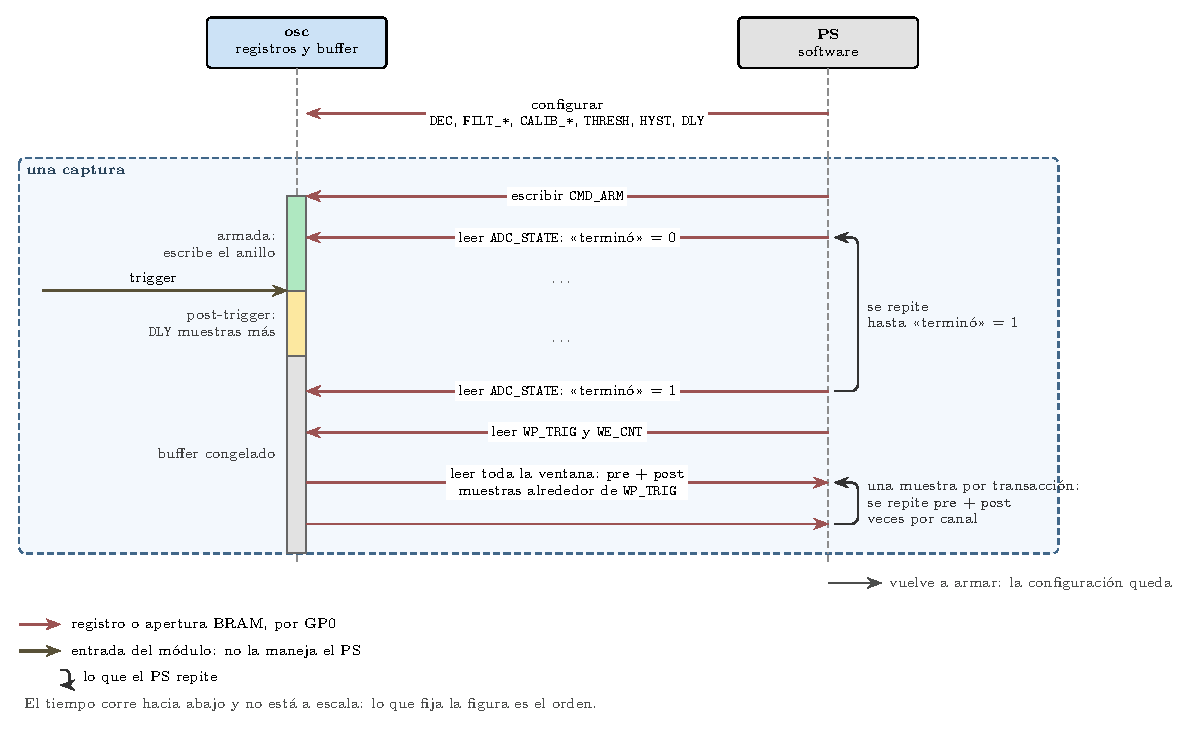
\includegraphics{cap8_secuencia_osc}
\caption[Secuencia de una captura del OSC básico]{%
Secuencia de una captura del OSC básico vista desde el PS, en modo single-shot
(\codigo{keep = 0}). El PS arma, sondea \codigo{ADC\_STATE} hasta que el buffer
queda congelado y recién entonces lee los punteros y la traza por el bus.
Mientras el PS lee, la captura está detenida.\label{f:osc-secuencia-basica}}
\end{figure}

Un sistema de adquisición ``continua'' realiza un loop en estas tres fases. El
sistema también aporta un registro de configuración \codigo{keep} (modo
continuo): con \codigo{keep=1} el buffer nunca se congela, y después de cada
post-trigger la escritura sigue y la FSM queda esperando el próximo trigger. Se
detiene escribiendo \codigo{keep=0} y esperando que el sistema se congele.

Para que no tengamos sobreescritura del buffer, tenemos que estar seguros de que
no tenemos triggers mientras realizamos la lectura. Esto puede ser el caso si
nosotros lanzamos el trigger de forma externa o por SW. En el caso de no tener
control sobre el trigger, el modo \codigo{keep} no es deseable, debido a que
podemos tener \emph{tearing}: bajo este efecto, una lectura del buffer puede
resultar de una cantidad arbitraria de capturas.

En la Fig.~\ref{f:osc-secuencia-basica} las flechas PS$\rightarrow$PL son
escrituras (la configuración y el \codigo{arm}) y las PL$\rightarrow$PS son
lecturas (el estado, y los punteros y el buffer una vez congelado). Todas las
transacciones se realizan mediante el ``handshake completo'' explicado en la
Sec.~\ref{S:intro-hw-transferencia}.

El ciclo completo (armar, esperar el congelado, leer la ventana y volver a
armar) tarda $\tau = \qty{252.7}{\micro\second}$ medido en placa, y lo domina
la lectura de la ventana de a una muestra por transacción
(\qty{45.6}{\micro\second} por canal). Mientras tanto el hardware no puede
capturar: es una cola de capacidad $K = 1$, y los eventos que llegan en ese
lapso no quedan registrados en ningún contador. La
Sec.~\ref{S:osc-anillo-eventos} presenta cómo se elimina esa espera.

%==============================================================================
\section{Cambios realizados en la versión básica del proyecto}
\label{S:osc-cambios}

Las diferencias principales fueron dos. Primeramente, \textbf{aislamos la cadena
de acondicionamiento y exportamos la cadena de triggering} a su propio módulo
\textbf{multitrigger}, explicado en el Cap.~\ref{C:multitrigger}. Por otro lado,
volcamos como salidas los pasos intermedios del DSP mediante la utilización de
tres seleccionadores llamados \textbf{mca}, \textbf{mtrg} y \textbf{osc}; estos
últimos pueden verse en la Fig.~\ref{f:osc-panorama-scope-mt} representados en
gris. En la Sec.~\ref{S:top-datapath} se presentan estas decisiones en más
detalle.

\begin{figure}[H]
\centering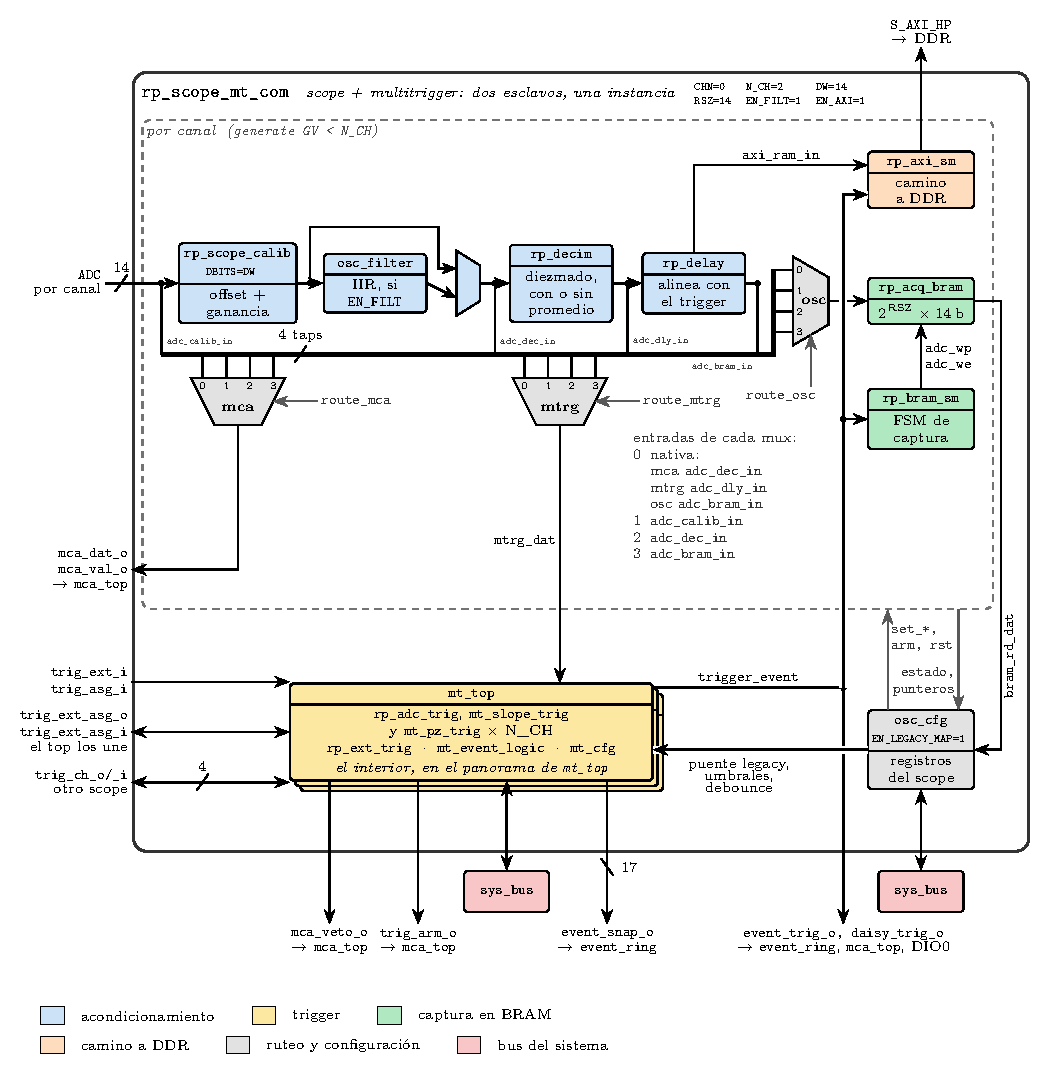
\includegraphics{cap8_panorama_scope_mt}
\caption[Módulo del scope utilizado en este proyecto]{%
Módulo del scope utilizado en este proyecto (\codigo{rp\_scope\_mt\_com}). La
cadena de triggering pasa a \codigo{mt\_top}, plegado (con sombra), y tres
\codigo{dsp\_tap\_mux} (en gris) eligen de qué nodo del DSP toma su muestra cada
consumidor: MCA, multitrigger y OSC. \codigo{trigger\_event} dispara a la vez la
captura de todos los canales, y todo corre en
\codigo{adc\_clk}.\label{f:osc-panorama-scope-mt}}
\end{figure}

%==============================================================================
\section{Versión anillo de eventos}
\label{S:osc-anillo-eventos}

El osciloscopio original de Red Pitaya cuenta con un camino de datos paralelo,
implementado en \codigo{rp\_axi\_sm} (no confundir con la
\codigo{rp\_bram\_sm}). En la Fig.~\ref{f:osc-deep-memory} se presenta el
mecanismo: después de un armado, las muestras se escriben de forma continua en
la memoria DDR del PS mediante la interfaz HP (en este camino el PL es master),
igual que en la BRAM, y tras el post-trigger la escritura se congela y se
actualizan los registros internos del módulo dentro del PL. Para averiguar en
qué sección de los 2~MB se encuentra el pulso, se tiene que realizar una
transacción de lectura al PL acerca de estas variables.

\begin{figure}[H]
\centering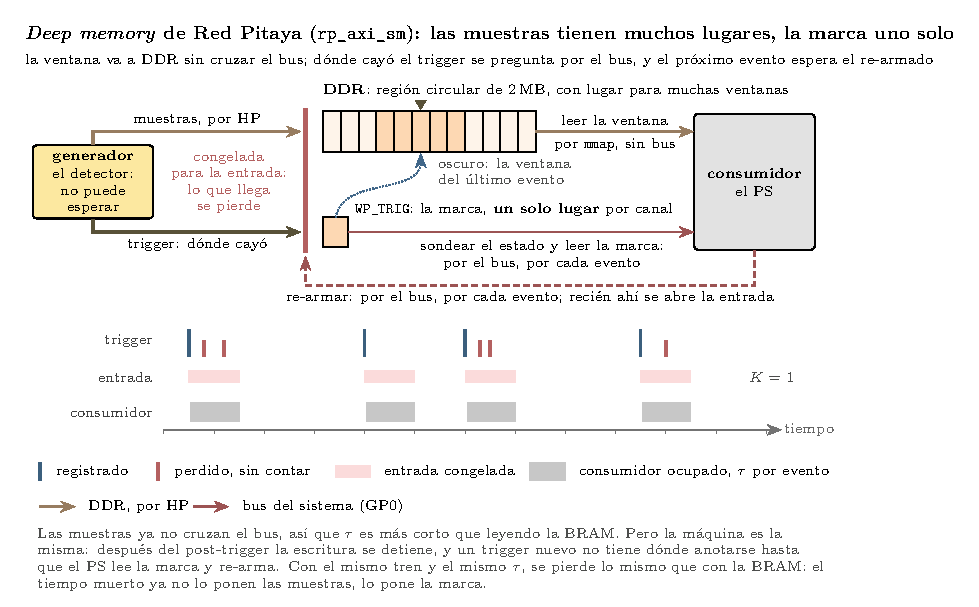
\includegraphics{cap8_deep_memory}
\caption[Esquema del \emph{deep memory} de Pitaya]{%
Esquema del \emph{deep memory} de Pitaya (\codigo{rp\_axi\_sm}) como generador,
buffer y consumidor. Las muestras van a DDR por HP, donde entran muchas
ventanas, pero dónde cayó el trigger se anota en un único registro
(\codigo{WP\_TRIG}). La entrada queda congelada hasta que el PS lo lee por el bus
y re-arma: se comporta como un buffer de $K = 1$. Es un esquema, no una
medición.\label{f:osc-deep-memory}}
\end{figure}

Esto parecería deseable, porque contamos con una región de memoria que puede
contener hasta $K$ eventos dentro de la misma, acercándonos a los requerimientos
de un sistema insensible a la latencia presentado en la
Sec.~\ref{S:intro-hw-latencia}. La gran diferencia entre este sistema y el
presentado es que el lector puede congelar el sistema aun teniendo toda la
memoria libre dentro del mismo. Este hecho hace que se comporte como uno con
$K=1$, debido a que la razón de existencia de este módulo es independizar ambos
extremos de la cola (o que queden únicamente asociados por la capacidad máxima
de la cola). Aun así, este sistema presenta mejoras con respecto al previo: no
tenemos que realizar un acceso palabra a palabra (32 bits) de la traza del
osciloscopio, así que reducimos el tiempo muerto por la transferencia de los
datos. Este tiempo es lineal con el largo de la transferencia, así que puede
ser muy útil si queremos obtener trazas considerablemente largas.

Este bloqueo se debe a que la presencia de un nuevo evento puede reescribir
cualquiera de los valores previos; esto \textbf{es considerar que la totalidad
del resto del buffer no se puede sobreescribir}, y no es necesariamente verdad.
Cada evento puede tomar una región de memoria dedicada en el buffer, de largo y
posición fija en DDR; esta región tiene en cuenta la segmentación del pulso en
hardware. La comparación entre el buffer segmentado y el original se presenta en
la Fig.~\ref{f:osc-ring-vs-buffer}. A cada región para un pulso la llamamos
casillero (\emph{slot}), y \textbf{contiene las variables de control que antes
transferíamos por GP0}. En la Fig.~\ref{f:osc-ring-vs-buffer}(b) se presenta su
estructura interna, que consiste en las regiones:
\begin{itemize}
  \item \textbf{Header} (cabecera): contiene los valores de metadata del
    evento; incluye el timestamp, la cantidad de canales, la cantidad de
    muestras, el número en la secuencia y el snapshot de trigger (qué trigger lo
    lanzó).
  \item \textbf{Datos+relleno}: contiene las muestras de la ventana más una
    región inválida para normalizar el ancho de los slots.
  \item \textbf{Footer}: es la marca de \emph{commit}: indica que el slot está
    completo. Si el slot se puede volver a escribir no lo dice el footer sino
    los créditos (\codigo{RD\_SLOT}).
\end{itemize}

\begin{figure}[H]
\centering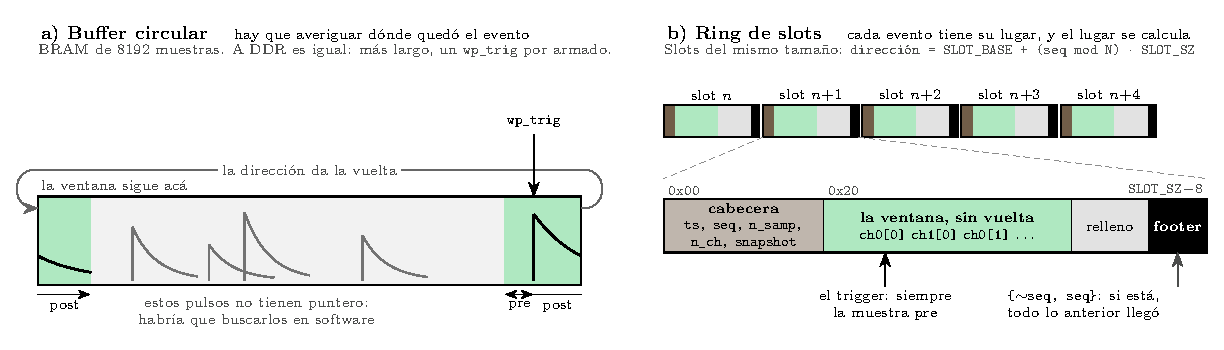
\includegraphics{cap8_ring_vs_buffer}
\caption[Dónde queda un evento en DDR: buffer circular y anillo de slots]{%
Dónde queda un evento en DDR. (a) Buffer circular: las muestras se escriben
corridas, y sólo el último evento tiene puntero (\codigo{wp\_trig}); los
anteriores habría que buscarlos en software. (b) Anillo de slots: cada evento
ocupa un slot de largo fijo, con cabecera, muestras, relleno y el footer
\codigo{\{\textasciitilde seq, seq\}}, y su dirección se calcula como
\codigo{SLOT\_BASE + (seq mod N)$\cdot$SLOT\_SZ}.\label{f:osc-ring-vs-buffer}}
\end{figure}

Esta implementación libera ancho de banda en el canal (no estamos transfiriendo)
y, mucho más importante, podemos subdividir la lectura del mismo en hasta la
cantidad de slots que deseemos. Este esquema de comunicaciones se suele
describir como \emph{descriptor ring}~\cite{Virtio12,Corbet2005}. A
continuación describimos cómo funciona la sección de control, vista desde el PS.

\subsection{Funcionamiento del footer}
\label{S:osc-footer}

Es una \textbf{marca de \emph{commit} al final del slot}: si no tiene el valor
esperado, el PS no lee el resto. Es el mecanismo habitual cuando un mensaje es
largo o su latencia es desconocida: se escribe el cuerpo y, al final, una marca
que confirma que todo lo anterior ya llegó. Como el PL escribe el slot en orden
de dirección, ver el footer con el \codigo{seq} esperado garantiza que la
cabecera y las muestras ya están en la DDR. El PS tampoco tiene que confirmar
cada evento: devuelve \textbf{créditos} publicando \codigo{RD\_SLOT} una vez por
lote, y el PL escribe de forma ininterrumpida mientras le queden créditos.

\subsection{Metodología de utilización del anillo}
\label{S:osc-uso-anillo}

En la Fig.~\ref{f:osc-secuencia-ring} se presentan las transacciones. Se habla
de lote porque se aprovecha que los elementos ya están en DDR para agruparlos en
regiones contiguas y así realizar movimientos de datos más eficientes. Para que
esto funcione de forma correcta tenemos que configurar los parámetros de la
región de memoria; estos sólo se latchean con la adquisición parada, y
escribirlos corriendo se ignora y levanta la flag \codigo{err\_cfg}. Incluyen:
\begin{enumerate}
  \item Tamaño \codigo{RING\_SZ} y posición de la región de DDR volátil (este
    tipo de acceso a memoria debe configurarse en el OS; el anillo usa la región
    de 32~MB en \codigo{0x0A00\_0000} que el proyecto de Pitaya reserva para el
    analizador lógico, y no la de 2~MB del \emph{deep memory}).
  \item Tamaño del \codigo{SLOT\_SHIFT}.
  \item Cantidad de slots, que no se escribe: el módulo la deriva como
    \codigo{N\_SLOTS = RING\_SZ \textgreater\textgreater{} SLOT\_SHIFT}. Todos
    deben entrar en la región DDR asignada.
  \item Tamaño de PRE y POST trigger de la ventana. La cabecera, la ventana y el
    footer deben entrar en un slot de $2^\text{SLOT\_SHIFT}$ bytes.
\end{enumerate}
Antes de escribir la geometría, el PS para el anillo, espera que llegue a
\codigo{STOPPED} y escribe \codigo{CTRL.clr}. Esto vacía el stage, el escritor
y el \codigo{axi\_wr\_fifo}, pone en cero \codigo{WR\_SLOT}, \codigo{RD\_SLOT},
\codigo{SEQ} y los contadores de descarte, y limpia \codigo{err\_cfg}. Después
el PS \textbf{pone en cero el footer de cada slot}, escribiendo directamente en
la DDR: el slot $k$ de la corrida anterior tiene el mismo \codigo{seq} que
tendrá el de esta, con un footer válido, y sin borrarlo la primera vuelta lo
entregaría como nuevo. Con una barrera de por medio escribe la geometría, la
relee (\codigo{N\_SLOTS}, \codigo{err\_cfg} y \codigo{WR\_SLOT = 0}) y recién
entonces activa el módulo con \codigo{CTRL.run} (ver la
Fig.~\ref{f:osc-fsm-ring}).

Por simplicidad, asociamos un único hilo de ejecución dentro del PS para este
módulo. El código del Cap.~\ref{C:sw} realiza lo siguiente:
\begin{enumerate}
  \item Lee \codigo{WR\_SLOT} por GP0 una vez por lote de eventos, para saber
    cuántos slots hay candidatos.
  \item Valida el footer de cada uno en la DDR. El primero que no está corta el
    bloque, porque \codigo{WR\_SLOT} avanza cuando el FIFO acepta el footer, no
    cuando el footer llega a la DDR.
  \item Pone una barrera de memoria, que ordena los accesos: garantiza que los
    footers se leyeron antes que los datos (ver la
    Sec.~\ref{S:hw-modelo-memoria}). Recién después lee la cabecera y las
    muestras.
  \item Pone otra barrera y publica \codigo{RD\_SLOT} una vez por bloque,
    devolviendo los créditos de todos sus slots.
\end{enumerate}
Con el buffer circular el trabajo era \textbf{por evento}, y la captura queda
congelada mientras el PS lee. Con el ring es \textbf{por lote} y la captura no
se detiene.

\begin{figure}[H]
\centering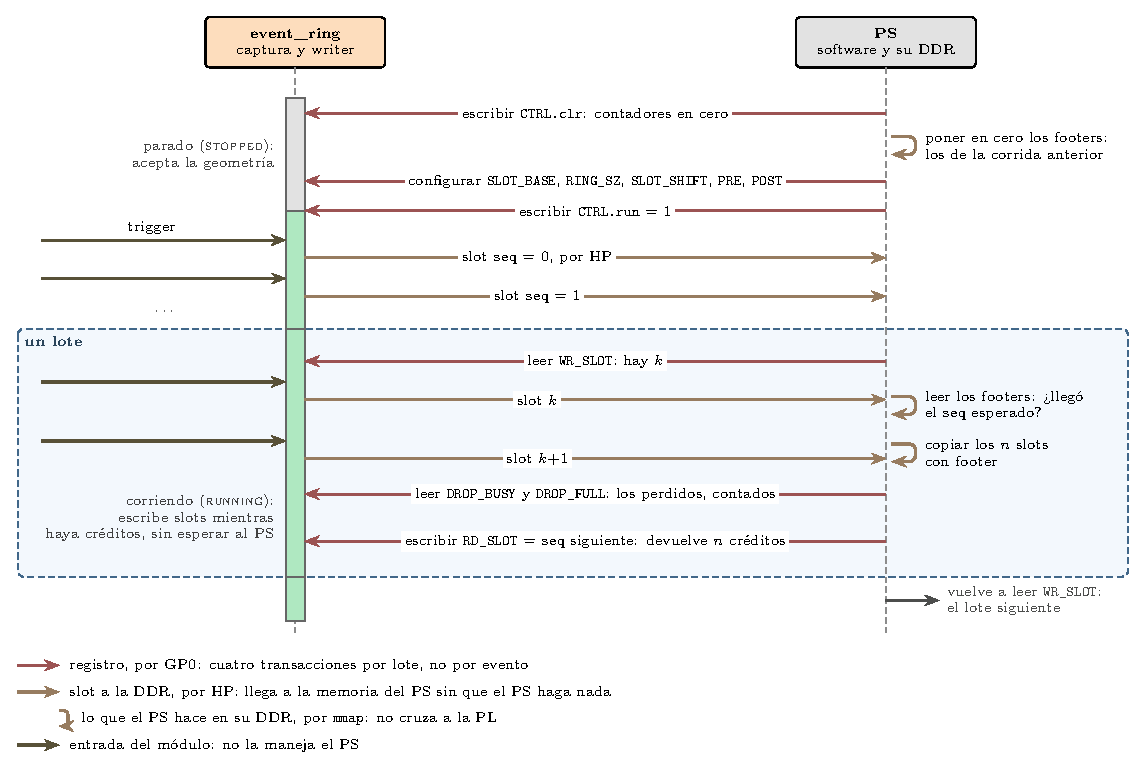
\includegraphics{cap8_secuencia_ring}
\caption[Flujo de utilización del anillo de eventos]{%
Flujo de utilización del anillo de eventos. Tenemos tres fases: (1)
inicialización, (2) arranque y (3) lectura por lote, con el commit dado por el
footer (\codigo{seq}) y el acknowledge por la escritura de
\codigo{RD\_SLOT}.\label{f:osc-secuencia-ring}}
\end{figure}

Si se quisiera, se podría sondear sólo el footer y no leer \codigo{WR\_SLOT}. La
diferencia es que sin \codigo{WR\_SLOT} el lazo no toca el GP0, pero el PS no
sabe cuántos slots hay listos y tiene que leer los footers de a uno hasta dar
con uno que no está. Con \codigo{WR\_SLOT}, una sola lectura por bloque
($\sim$\qty{2.3}{\micro\second}, repartidos entre todos los eventos del bloque)
dice cuántos pedir, y el commit lo sigue dando el footer.

En la siguiente sección mostramos la vista general del módulo que implementa la
comunicación mediante el anillo.

\subsection{Panorama del módulo del anillo}
\label{S:osc-panorama-anillo}

El anillo reemplaza al camino a DDR original: \codigo{rp\_axi\_sm} queda
deshabilitado (\codigo{EN\_AXI = 0}) y en su lugar se usa
\codigo{event\_ring\_top}, con las conexiones de la
Fig.~\ref{f:osc-panorama-scope-ring}. En el bitstream el anillo no está dentro
del scope sino en el TOP, al lado de él, con esas mismas conexiones. Se dejó el
camino original por AXI\_GP0 y la BRAM porque la versión original del módulo
contenía ambos caminos, y por compatibilidad del mapa de registros.

\begin{figure}[H]
\centering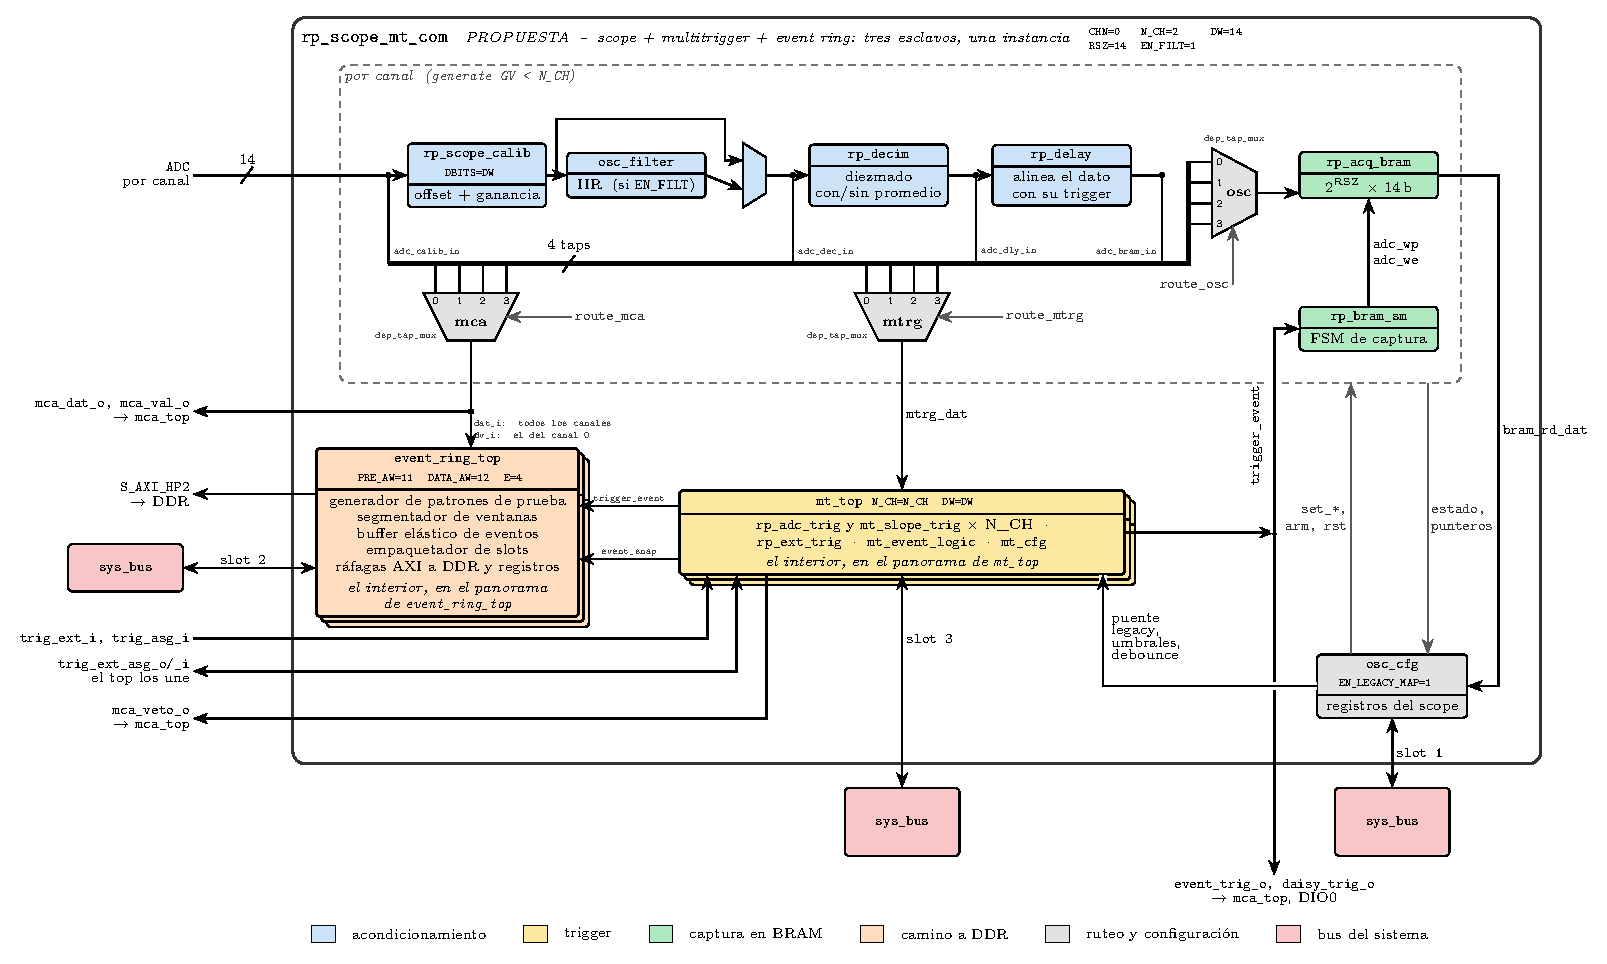
\includegraphics{cap8_panorama_scope_ring}
\caption[Conexión del anillo de eventos con el scope]{%
Conexión del anillo de eventos con el scope. \codigo{event\_ring\_top} toma el
lugar de \codigo{rp\_axi\_sm}, el camino a DDR. La BRAM se mantiene porque es la
que leen \codigo{librp} y la secuencia del OSC básico. Los bloques con sombra
están plegados: su interior está en los panoramas de \codigo{mt\_top} y
\codigo{event\_ring\_top}. En el bitstream el anillo se instancia en el TOP, al
lado del scope, con estas mismas conexiones.\label{f:osc-panorama-scope-ring}}
\end{figure}

%==============================================================================
\section{Funcionamiento del módulo de ring de eventos}
\label{S:osc-ring-funcionamiento}

En la Fig.~\ref{f:osc-freno-descarte} se puede ver la cadena principal del
datapath del módulo de ring de eventos \codigo{event\_ring\_top}, que contiene
los siguientes submódulos:
\begin{itemize}
  \item \codigo{event\_window\_capture}: es el que segmenta las muestras de la
    entrada en las trazas correspondientes a subir al FIFO.
  \item \codigo{event\_stage\_fifo}: es un \textbf{buffer
    elástico}~\cite{Cortadella2006} que guarda todas las fuentes de datos de un
    evento en buffers separados.
  \item \codigo{event\_slot\_writer}: arma la trama de bits que representa un
    slot a partir de los datos de los buffers de la etapa anterior, es decir,
    serializa un evento a un slot del anillo en DDR. Sale por la misma interfaz
    simplificada de Instrumentation Technologies que usaba
    \codigo{rp\_axi\_sm}, para seguir el formato del sistema original.
  \item \codigo{axi\_wr\_fifo}: módulo de paquetizado del proyecto original de
    Pitaya, requerido para pasar a la interfaz HP2, del tipo AXI-Full. A este no
    se lo describirá porque no fue parte de este proyecto; para más información
    se refiere a la documentación oficial de Pitaya~\cite{RedPitayaFPGA}.
\end{itemize}

\begin{figure}[H]
\centering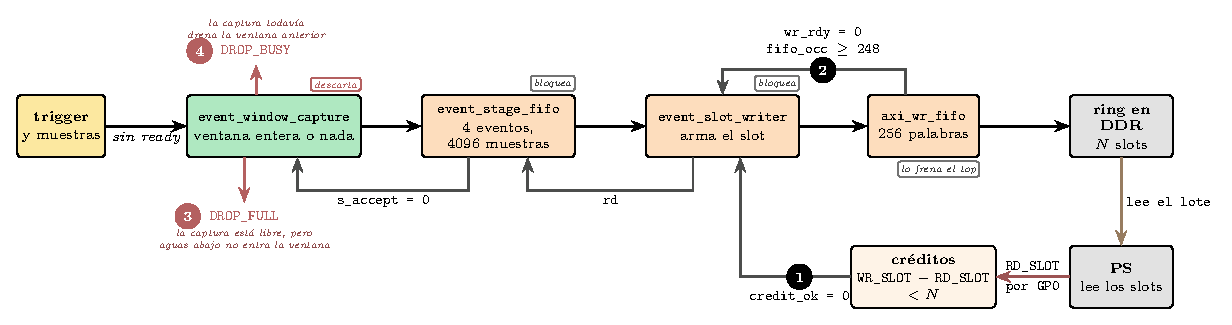
\includegraphics{cap8_ring_freno_descarte}
\caption[Dónde se frena y dónde se descarta en el anillo]{%
Dónde se frena y dónde se descarta en el anillo cuando algo no alcanza. Sólo la
captura descarta, porque el trigger y las muestras le llegan sin
\codigo{ready}: el evento que no puede tomar lo pierde entero y lo cuenta
(flecha roja). El stage y el escritor sólo bloquean, y su contrapresión
(flechas de vuelta) sube hasta la captura sin perder datos. Los números son las
filas de la Tabla~\ref{t:osc-freno-descarte}.\label{f:osc-freno-descarte}}
\end{figure}

Como explicamos en la Sec.~\ref{S:intro-hw-back-pressure}, la cantidad de
eventos perdidos en toda la cadena es igual a la \textbf{suma de eventos
perdidos en cada una de las etapas individuales}, si lo expandimos al sistema
actual.

Si analizamos la composición interna del módulo, además de la cadena principal
(en naranja claro) identificamos las siguientes cinco secciones de lógica
propias del top:
\begin{itemize}
  \item \textbf{Submódulo de configuración}: sección compartida explicada en la
    Sec.~\ref{S:intro-hw-modulo-config}.
  \item \textbf{Timestamp}: contador de 64 bits que avanza con cada
    \codigo{dv}. Vuelve a 0 en \codigo{STOPPED}, así que $t = 0$ es el arranque
    de la corrida. La captura lo copia en la cabecera de cada evento.
  \item \textbf{Créditos}: calcula los slots ocupados en la DDR como
    \codigo{wr\_slot $-$ rd\_slot}, así que funciona aunque los contadores den
    la vuelta. \codigo{credit\_ok = ocupados \textless{} N\_slots}.
    \codigo{rd\_slot} lo publica el PS cuando termina de leer un lote. Sin
    crédito, el writer espera para no pisar un slot que el PS todavía no leyó.
  \item \textbf{Dirección}: indica los valores límite dados los registros de
    configuración internos, stop = \codigo{SLOT\_BASE + RING\_SZ $-$ 8}.
  \item \textbf{Contrapresión}: calcula una ocupación propia del
    \codigo{axi\_wr\_fifo} por el master. Hace falta porque el FIFO del
    proyecto de Pitaya no expone su nivel y \textbf{descarta en silencio si se
    pushea estando lleno}. Si aun así el FIFO desborda, queda un sticky
    \codigo{err\_fifo\_ovf}.
\end{itemize}

\begin{figure}[H]
\centering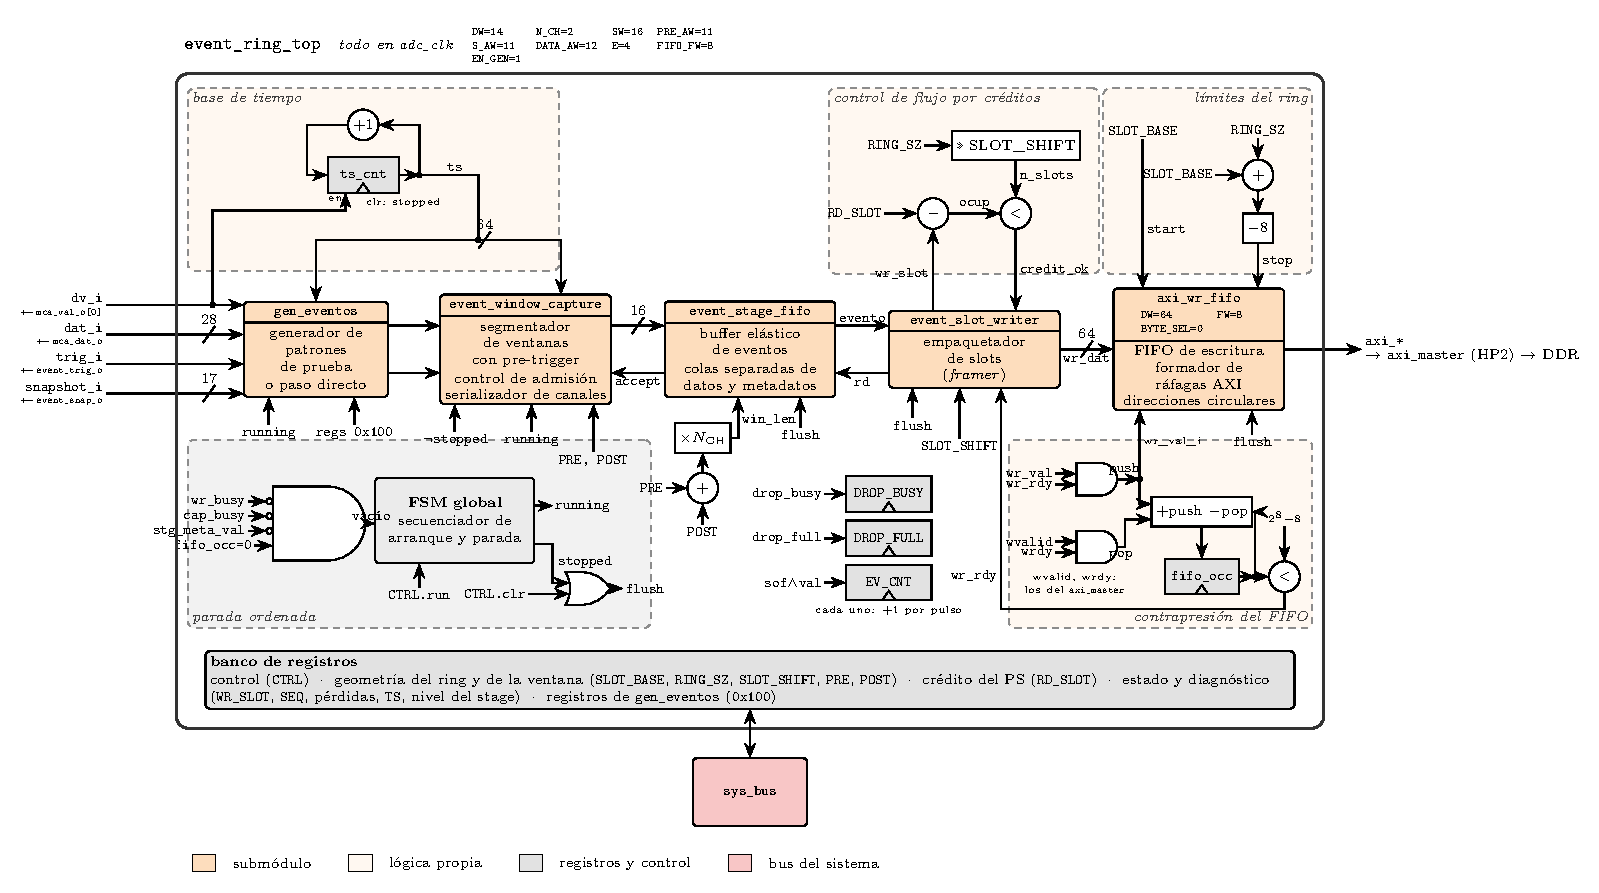
\includegraphics{cap8_panorama_event_ring_top}
\caption[Estructura interna de \codigo{event\_ring\_top}]{%
Estructura interna de \codigo{event\_ring\_top}. Contiene la cadena de la
Fig.~\ref{f:osc-freno-descarte} (en naranja claro) y la lógica propia del top:
configuración, timestamp, créditos, dirección, contrapresión y FSM global. El
PS no lee ningún registro por evento: lee \codigo{WR\_SLOT} y publica
\codigo{RD\_SLOT} una vez por lote, y valida cada slot por su footer en DDR.
\codigo{gen\_eventos} está entre la entrada y la captura; apagado, es un paso
directo.\label{f:osc-panorama-ring-top}}
\end{figure}

Nos quedó por explicar el \textbf{manejo de la FSM}: en la
Fig.~\ref{f:osc-fsm-ring} se puede observar una FSM global de tres estados
(\codigo{STOPPED}, \codigo{RUNNING}, \codigo{DRAINING}). En \codigo{STOPPED} se
vacían el stage, el escritor y el \codigo{axi\_wr\_fifo}, y se ponen en cero
\codigo{wr\_slot}, \codigo{rd\_slot} y el timestamp; es el único estado en que
se acepta la geometría. En \codigo{RUNNING} la captura acepta triggers. Al bajar
\codigo{CTRL.run} pasa a \codigo{DRAINING}: la captura no acepta triggers nuevos
pero termina la ventana en vuelo, y vuelve a \codigo{STOPPED} recién cuando la
captura y el escritor están libres, el stage no tiene eventos y el
\codigo{axi\_wr\_fifo} largó su última palabra. Así una parada nunca deja un
slot sin su footer.

\begin{figure}[H]
\centering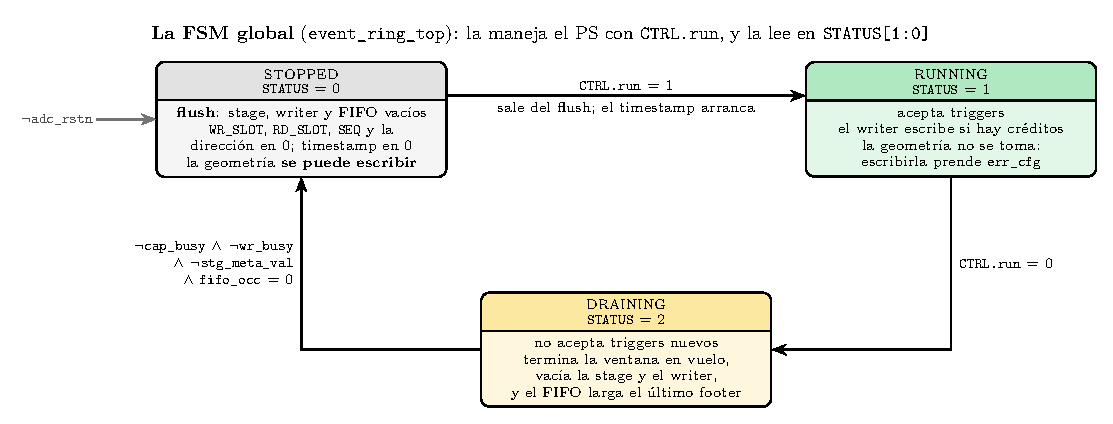
\includegraphics{cap8_fsm_event_ring_top}
\caption[FSM global del anillo de eventos]{%
FSM global del anillo de eventos, que el PS maneja con \codigo{CTRL.run} y lee
en \codigo{STATUS[1:0]}. \codigo{DRAINING} deja terminar la ventana en vuelo y
vacía la cadena antes de volver a \codigo{STOPPED}. Si se para con el anillo
lleno, no termina hasta que el PS devuelve créditos o escribe
\codigo{CTRL.clr}. Llegar a \codigo{STOPPED} pone en cero los contadores de
slot.\label{f:osc-fsm-ring}}
\end{figure}

\subsection{Cálculo de tiempo muerto y contadores presentes}
\label{S:osc-tiempo-muerto}

Recordemos que el tiempo muerto es el tiempo durante el cual el sistema no puede
aceptar un evento nuevo; los eventos que llegan en ese lapso se pierden. En la
Fig.~\ref{f:osc-freno-descarte} se presentan todas las etapas principales del
anillo de eventos implementado. Todas las etapas cuentan con una conexión
trasera con la cual emiten la disponibilidad del módulo a una nueva
transacción; este es un bloqueo controlado del flujo de datos.

Es importante notar que la etapa que toma en cuenta los créditos no es la que
tiene conexión directa con la interfaz AXI, el \codigo{axi\_wr\_fifo}, sino la
penúltima, \codigo{event\_slot\_writer}. Esto se debe a que
\codigo{axi\_wr\_fifo} es un paquetizador: no tiene en cuenta el mecanismo de
transferencia de datos implícito en el módulo (la versión expandida que
referenciamos al final de la Sec.~\ref{S:intro-hw-transferencia}). Si
describimos en más detalle todos estos pasos, nos vamos a encontrar con la
información presentada en la Tabla~\ref{t:osc-freno-descarte}.

\begin{table}[H]
\centering
\caption[Recursos que pueden agotarse en el anillo]{%
Recursos que pueden agotarse en el anillo, la señal que lo indica y qué pasa en
cada caso. Los niveles 1 y 2 \textbf{frenan} al escritor sin perder datos; los 3
y 4 \textbf{descartan} el evento entero en la captura y lo cuentan en
\codigo{DROP\_FULL} y \codigo{DROP\_BUSY}.\label{t:osc-freno-descarte}}
\small
\begin{tabularx}{\textwidth}{|c|>{\raggedright\arraybackslash}p{0.27\textwidth}%
  |l|>{\raggedright\arraybackslash}X|}
\hline \encabezado \textbf{Nivel} & \textbf{Recurso} & \textbf{Señal} &
  \textbf{Qué pasa al agotarse} \\ \hline
1 & slots de DDR & \codigo{credit\_ok} & el writer \textbf{se frena} en
  \codigo{W\_IDLE} \\ \hline
2 & \codigo{axi\_wr\_fifo} & \codigo{wr\_rdy} & el writer \textbf{se frena} a
  mitad de slot \\ \hline
3 & stage (muestras + metadatos) & \codigo{s\_accept} & la captura
  \textbf{descarta entero} $\rightarrow$ \codigo{drop\_full} \\ \hline
4 & la captura misma & \codigo{busy} & trigger durante el drenaje
  $\rightarrow$ \codigo{drop\_busy} \\ \hline
\end{tabularx}
\end{table}

%==============================================================================
\section{Detalles de submódulos}
\label{S:osc-submodulos}

\subsection{Módulo de captura de ventana:
\texorpdfstring{\texttt{event\_window\_capture}}{event\_window\_capture}}
\label{S:osc-window-capture}

Reemplaza el rol de \codigo{rp\_bram\_sm}. Este módulo es común a todos los
slots, y su funcionalidad consiste en que por cada \textbf{trigger se extrae una
ventana de muestras como un AXI-Stream}; la misma incluye \codigo{pre} antes y
\codigo{post} desde el disparo.
\begin{itemize}
  \item Tiene \textbf{una sola memoria}, el pre-buffer: un buffer circular de
    $2^{11}$ palabras que se escribe siempre y del que salen tanto el pre como
    el post. Los metadatos del evento (\codigo{m\_ts}, \codigo{m\_snap},
    \codigo{m\_nsamp}) se guardan en tres registros.
  \item El evento se acepta o se descarta entero; esto se decide en el ciclo del
    trigger, antes de emitir el \emph{start of frame} (SOF).
\end{itemize}

Tenemos una segmentación de las ventanas de captura mediante la utilización de
símbolos que representan el inicio de una ventana, llamado \emph{start of frame}
(SOF), y el final de la ventana, llamado \emph{end of frame} (EOF). La FSM del
sistema se presenta en la Fig.~\ref{f:osc-fsm-window}; lo más importante es que
mueve \textbf{sólo el lado de lectura del pre-buffer} y consta de tres estados.

Con \codigo{run\_i} en 1, cada \codigo{dv} (data valid) escribe una palabra y
avanza \codigo{wr\_ptr}, en cualquier estado.

La señal \codigo{m\_accept} la da \codigo{event\_stage\_fifo}, indica si tiene
lugar disponible y se mira únicamente en el ciclo de trigger:
\begin{enumerate}
  \item \codigo{IDLE}: espera el trigger.
  \begin{itemize}
    \item Si el stage no tiene lugar (\codigo{m\_accept\_i = 0}), sale un pulso
      de \codigo{drop\_full\_o} y la FSM se queda en \codigo{ST\_IDLE}.
    \item Si tiene lugar, en el mismo ciclo carga
      \codigo{rd\_ptr $\leftarrow$ wr\_ptr $-$ pre},
      \codigo{samp\_left $\leftarrow$ pre + post} y los metadatos
      (\codigo{m\_ts}, \codigo{m\_snap} y \codigo{m\_nsamp}), pone
      \codigo{ch\_idx} y \codigo{word\_val} en 0, y pasa a
      \codigo{ST\_DRAIN}.
  \end{itemize}
  \item \codigo{DRAIN}: \textbf{copia la ventana}; cada ciclo hace dos tareas al
    mismo tiempo:
  \begin{enumerate}
    \item \textbf{Leer}: si no hay palabra cargada, o la cargada está entregando
      su último canal, y \codigo{rd\_ptr $\neq$ wr\_ptr}, lee
      \codigo{pre\_buf[rd\_ptr]} en \codigo{word\_r} y avanza
      \codigo{rd\_ptr}. Durante el pre siempre hay dato (se arrancó
      \codigo{pre} atrás); durante el post, la comparación espera a que llegue
      la muestra siguiente.
    \item \begin{sloppypar}\textbf{Serializar}: con palabra cargada saca un canal por ciclo
      (\codigo{m\_dat\_o} $\leftarrow$ \codigo{word\_r[ch\_idx]}) y avanza
      \codigo{ch\_idx}; con el último canal descuenta \codigo{samp\_left}.
      \codigo{m\_sof\_o} sale con el canal 0 de la primera muestra y
      \codigo{m\_eof\_o} con el último canal de la última, y ahí pasa a
      \codigo{ST\_TAIL}. Un trigger en este estado no se acepta: sale un pulso
      de \codigo{drop\_busy\_o}.\end{sloppypar}
  \end{enumerate}
  \item \codigo{TAIL}: \textbf{dura un ciclo}; deja que \codigo{m\_eof\_o}
    salga por su registro antes de aceptar un trigger nuevo (un trigger en este
    ciclo también se cuenta como \codigo{drop\_busy}), y vuelve a
    \codigo{ST\_IDLE}. La captura queda ocupada
    $(\text{pre}+\text{post})\cdot N_\text{CH} + 2$ ciclos después del trigger
    aceptado, así que dos triggers sólo se aceptan si están separados al menos
    $2S+3$ ciclos (con $S$ = \codigo{pre+post} y $N_\text{CH}=2$), que es la
    ventana ciega que medimos en placa. Esto vale sin diezmado (\codigo{dv} en
    todos los ciclos); con diezmado $D$ el post llega a una muestra cada $D$
    ciclos y la ventana dura aproximadamente $\text{post}\cdot D$ ciclos más el
    pre.
\end{enumerate}

\begin{figure}[H]
\centering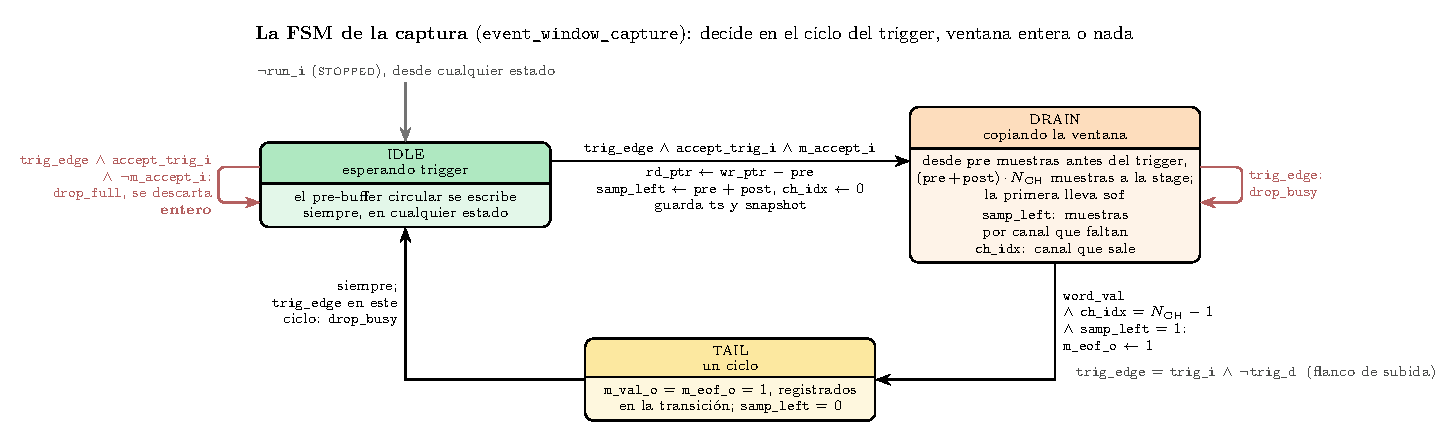
\includegraphics{cap8_fsm_window_capture}
\caption[FSM de captura de un evento]{%
FSM de captura de un evento (\codigo{event\_window\_capture}). Mueve sólo el
lado de lectura del pre-buffer; la escritura sigue en cualquier estado.
\codigo{m\_accept\_i} se mira una sola vez, en el ciclo del trigger: sin lugar,
el evento se descarta entero (\codigo{drop\_full}), y un trigger en
\codigo{DRAIN} o \codigo{TAIL} se pierde como \codigo{drop\_busy}. Con el
anillo en \codigo{RUNNING} todo flanco queda contado:
\codigo{EV\_CNT + DROP\_BUSY + DROP\_FULL} = triggers.\label{f:osc-fsm-window}}
\end{figure}

Mientras que en la Fig.~\ref{f:osc-panorama-window} podemos identificar:
\begin{enumerate}
  \item \textbf{Flanco y decisión} (amarillo):
  \begin{enumerate}
    \item \codigo{trig\_d} guarda el trigger del ciclo anterior y
      \codigo{trig\_edge = trig\_i $\land$ $\lnot$trig\_d}: se toma el flanco y
      no el nivel, porque el disparo por software puede durar más de un ciclo
      de \codigo{adc\_clk} (en placa daba dos eventos por disparo).
    \item \codigo{trig\_edge $\land$ accept\_trig\_i $\land$ idle} es un trigger
      que la captura puede tomar; con \codigo{m\_accept\_i} se separa en
      \codigo{acepta} (carga punteros y metadatos, arranca la FSM) o
      \codigo{drop\_full} (sin lugar aguas abajo, el evento se descarta
      entero).
    \item Un \codigo{trig\_edge} con \codigo{busy} da \codigo{drop\_busy}.
  \end{enumerate}
  \item \textbf{Metadatos} (gris, arriba a la derecha): cuando tenemos
    \codigo{acepta} en alto carga tres registros:
    \codigo{m\_ts $\leftarrow$ ts\_i}, \codigo{m\_snap $\leftarrow$ snapshot\_i}
    y \codigo{m\_nsamp $\leftarrow$ pre\_i + post\_i}, el largo por canal.
  \item \textbf{FSM de ventana} (gris, en el centro): es la de la
    Fig.~\ref{f:osc-fsm-window}.
  \item \textbf{Manejo de punteros y el pre-buffer} (azul):
  \begin{enumerate}
    \item Tenemos una extensión de signo previa de 14 a 16 bits por canal (la
      palabra de los dos canales pasa de 28 a 32 bits).
    \item Se escribe \codigo{pre\_buf[wr\_ptr]} en cada ciclo con
      \codigo{run\_i} y \codigo{dv\_i} en 1.
    \item \codigo{wr\_ptr} suma 1 con cada \codigo{dv\_i}.
    \item El comparador \codigo{rd\_ptr $\neq$ wr\_ptr} da
      \codigo{rd\_avail}.
  \end{enumerate}
  \item \textbf{Pedir palabra}: decide en qué ciclo se lee el pre-buffer. Cada
    palabra trae las $N_\text{CH}$ muestras de un instante, pero la salida
    entrega una por ciclo, así que una palabra alcanza para $N_\text{CH}$
    ciclos.
  \begin{enumerate}
    \item Se pide una palabra cuando no hay ninguna pendiente de serializar
      (\codigo{$\lnot$word\_val}), o cuando la pendiente está entregando su
      último canal (\codigo{ch\_last}): como la lectura tarda un ciclo, la
      palabra nueva llega justo a tiempo y el stream no tiene huecos.
    \item La lectura se hace sólo si hay dato
      (\codigo{do\_read = want\_word $\land$ rd\_avail}); en el post espera a
      que llegue la muestra siguiente.
  \end{enumerate}
  \item \textbf{Contadores de la ventana}: dos registros que usan las regiones
    de pedir palabra y del serializador.
  \begin{enumerate}
    \item \codigo{word\_val}: hay palabra pendiente si se acaba de leer una, o si
      la que estaba todavía tiene canales por entregar.
    \item \codigo{samp\_left}: se carga con \codigo{pre + post} al aceptar y
      baja en uno con cada palabra terminada. Con
      \codigo{samp\_left = m\_nsamp} sale el SOF y con
      \codigo{samp\_left = 1} el EOF; en 0 deja de pedir.
  \end{enumerate}
  \item \textbf{Serializador}:
  \begin{enumerate}
    \item \codigo{word\_r} guarda la palabra leída del pre-buffer (las
      $N_\text{CH}$ muestras de un instante) y un mux elegido por
      \codigo{ch\_idx} saca un canal por ciclo. \codigo{m\_val},
      \codigo{m\_dat}, \codigo{m\_sof} y \codigo{m\_eof} van registrados
      juntos; \codigo{m\_sof} sale con \codigo{ch\_idx = 0} y
      \codigo{samp\_left = m\_nsamp}, y \codigo{m\_eof} con \codigo{ch\_last} y
      \codigo{samp\_left = 1}.
    \item El stream queda con los canales intercalados:
      \codigo{ch0[k], ch1[k], ch0[k+1], \ldots}.
    \item Como se lee una palabra cada $N_\text{CH}$ ciclos y se escribe una por
      ciclo, el rezago entre punteros crece hasta
      $(\text{pre}+\text{post})\cdot N_\text{CH} - \text{post}$. Con $2^{11}$
      palabras entra cualquier ventana de hasta 1024 muestras con
      \codigo{pre} $\leq$ 1023; el bloque no lo verifica, por eso el límite lo
      impone la configuración.
  \end{enumerate}
\end{enumerate}

\begin{figure}[H]
\centering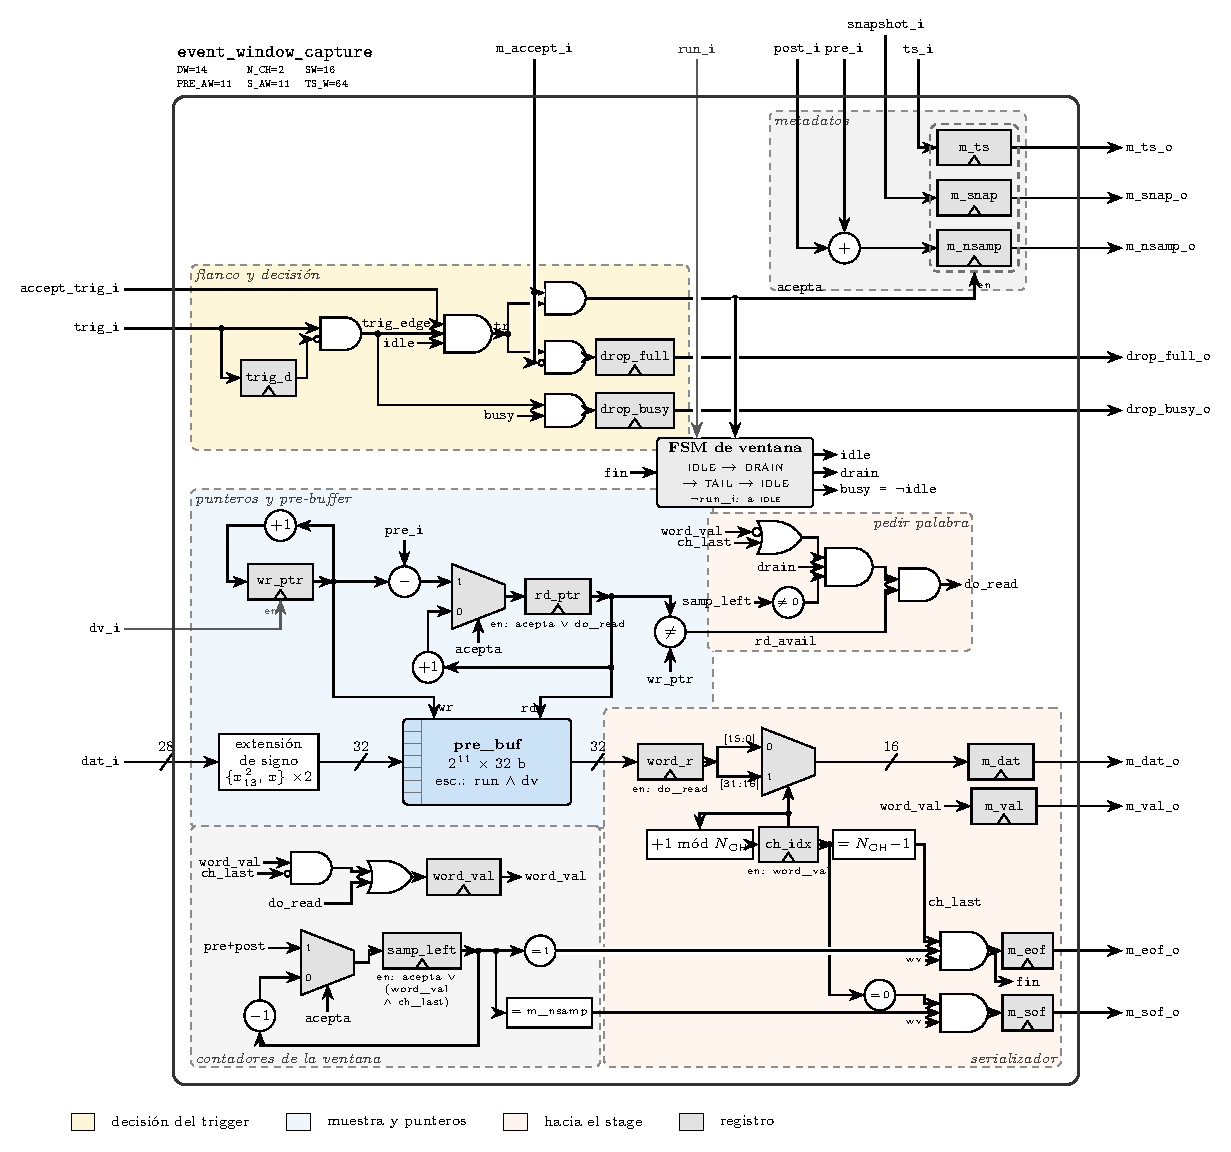
\includegraphics{cap8_panorama_window_capture}
\caption[Vista general de \codigo{event\_window\_capture}]{%
Vista general de \codigo{event\_window\_capture} a nivel de operación. Una sola
memoria guarda el pre y el post: al aceptar, \codigo{rd\_ptr} arranca
\codigo{pre} palabras atrás de \codigo{wr\_ptr}. Desde ahí se lee una palabra
cada $N_\text{CH}$ ciclos mientras el pre-buffer se sigue escribiendo a una por
ciclo. El serializador saca un canal por ciclo con un mux elegido por
\codigo{ch\_idx}. Las redes con nombre se conectan por nombre (\codigo{wv} =
\codigo{word\_val}), y \codigo{NOMBRE=valor} son los parámetros con que lo
instancia \codigo{event\_ring\_top}.\label{f:osc-panorama-window}}
\end{figure}

La FSM de la ventana es muy parecida a la presentada en la
Fig.~\ref{f:ap-osc-fsm-bram}, debido a que tiene el mismo objetivo: segmentar
con un trigger en la entrada un evento dado. Las diferencias ahora son:
\begin{enumerate}
  \item No tenemos un estado de ``armado'', sino que ese bit de información
    (armado/desarmado), que representaba si podíamos sobreescribir el buffer
    interno de los datos, se presenta como entrada del módulo en la señal
    \codigo{m\_accept\_i}: hay lugar aguas abajo para la ventana entera. La
    entrada \codigo{accept\_trig\_i} es otra cosa: la da la FSM global y vale 1
    sólo en \codigo{RUNNING}.
  \item El buffer no se congela: el pre-buffer se escribe siempre y la ventana
    se copia a un stream, así que la captura vuelve a estar lista sin
    intervención del PS.
\end{enumerate}

\subsection{Buffer elástico:
\texorpdfstring{\texttt{event\_stage\_fifo}}{event\_stage\_fifo}}
\label{S:osc-stage-fifo}

Este buffer elástico se denomina \emph{stage} porque no guarda únicamente las
muestras del evento, sino que también tiene una cola de metadatos; las mismas
\textbf{en esta instancia se encuentran desacopladas}. En la
Fig.~\ref{f:osc-panorama-stage} se presenta un diagrama de la misma, que
incluye:
\begin{itemize}
  \item \textbf{Cola de metadatos}: $E = 4$ entradas, con dos punteros
    \codigo{meta\_wr} y \codigo{meta\_rd}; se exporta el nivel presente
    \codigo{ev\_lvl\_o}. El metadato se escribe en el SOF, pero el evento
    \textbf{recién cuenta en el EOF}: \codigo{meta\_lvl} cuenta sólo eventos
    completos y \codigo{meta\_open} marca el que está entrando. Así el escritor
    nunca ve un evento cuyas muestras todavía están llegando, que podría drenar
    más rápido de lo que entran.
  \item \textbf{Cola de muestras}: $2^{12}$ muestras de 16 bits en BRAM, con
    punteros \codigo{wr\_ptr}/\codigo{rd\_ptr} y nivel \codigo{lvl}; cuenta
    cada muestra que entra y sale. La salida está registrada en
    \codigo{dout\_r}, así que la muestra vale un ciclo después del pop.
  \item \textbf{Criterio de aceptación}: requerimos espacio en ambas colas. Con
    \codigo{free \textgreater= win\_len\_i} comprobamos que tenemos el
    suficiente espacio en \codigo{mem}, mientras que \codigo{meta\_full} indica
    si la cola de metadatos puede almacenar otro evento, contando el que está a
    medio entrar.
\end{itemize}

\begin{figure}[H]
\centering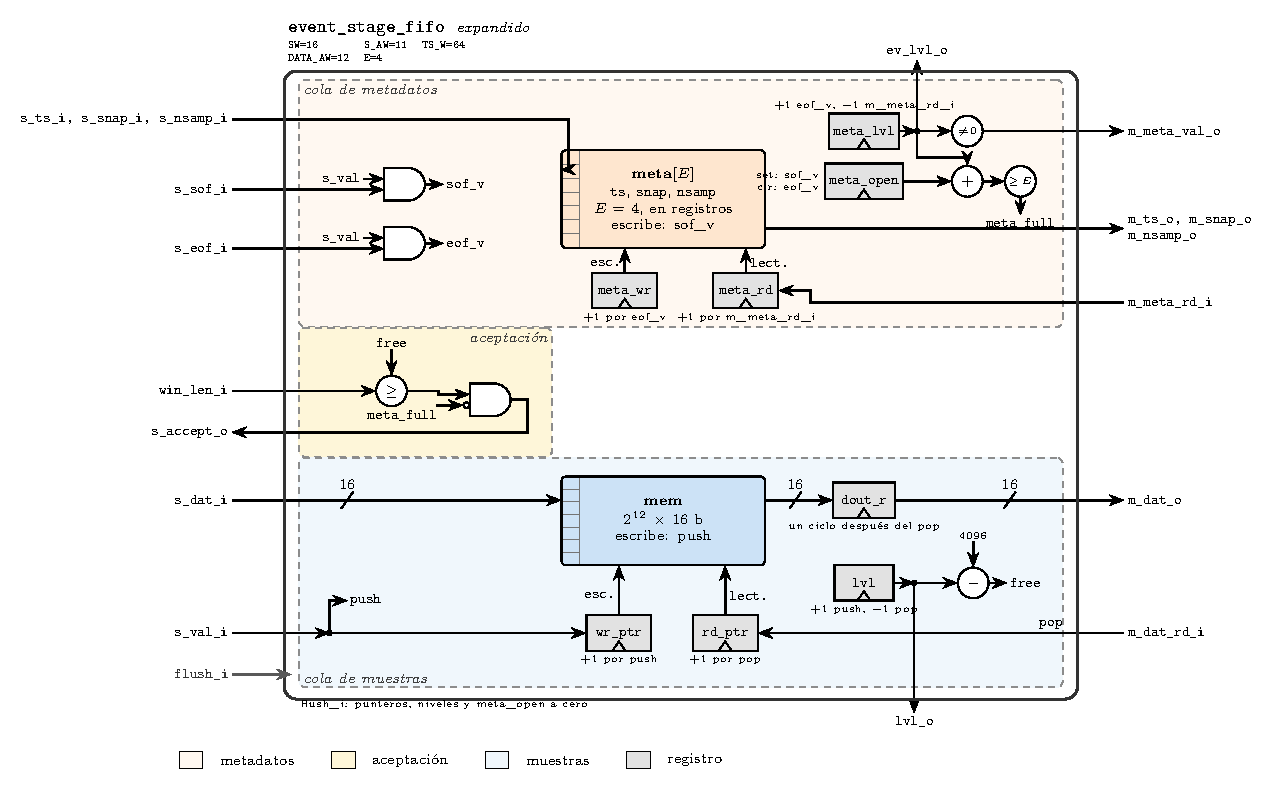
\includegraphics{cap8_panorama_stage_fifo}
\caption[Vista general de \codigo{event\_stage\_fifo}]{%
Vista general de \codigo{event\_stage\_fifo} a nivel de operación. El metadato
se escribe con el SOF, pero el evento recién cuenta con el EOF; así el escritor
no ve un evento cuyas muestras todavía están entrando. Para aceptar hace falta
lugar para la ventana entera y un lugar de metadato, contando el evento a medio
entrar: \codigo{s\_accept\_o = (free $\geq$ win\_len\_i) $\land$
$\lnot$meta\_full}. Con ventanas de 1024 muestras entran dos eventos, no
cuatro.\label{f:osc-panorama-stage}}
\end{figure}

\subsection{Módulo de escritura:
\texorpdfstring{\texttt{event\_slot\_writer}}{event\_slot\_writer}}
\label{S:osc-slot-writer}

Este módulo serializa un evento a un slot del anillo en DDR. Tiene como salida
un AXI-Stream clásico \{\codigo{wr\_data}, \codigo{wr\_val}, \codigo{wr\_rdy}\}
de 64 bits, y escribe exactamente $2^{\text{SLOT\_SHIFT}-3}$ palabras por
evento, en orden de dirección creciente, para que el generador lineal de
direcciones del \codigo{axi\_wr\_fifo} las coloque sin saltos. El layout del
slot se presenta en la Tabla~\ref{t:osc-layout-slot}.

\begin{table}[H]
\centering
\caption[Layout de un slot del anillo en DDR]{%
Layout de un slot del anillo en DDR. Las cuatro primeras palabras (32~B) son la
cabecera, y la cuarta está reservada.\label{t:osc-layout-slot}}
\small
\begin{tabularx}{\textwidth}{|l|>{\raggedright\arraybackslash}X|}
\hline \encabezado \textbf{Offset} & \textbf{Contenido} \\ \hline
\codigo{0x00} & \codigo{timestamp[63:0]}: ticks desde el arranque de la
  corrida \\ \hline
\codigo{0x08} & \codigo{\{flags[7:0], n\_ch[7:0], n\_samp[15:0],
  seq[31:0]\}} \\ \hline
\codigo{0x10} & \codigo{\{32'b0, 15'b0, snapshot[16:0]\}}: qué fuente
  disparó \\ \hline
\codigo{0x18} & reservado (0) \\ \hline
\codigo{0x20} \ldots & muestras int16, 4 por palabra, canales
  \textbf{intercalados}: \codigo{ch0[k], ch1[k], ch0[k+1], \ldots} \\ \hline
\ldots & relleno de ceros hasta la anteúltima palabra \\ \hline
\codigo{SLOT\_SZ $-$ 8} & \textbf{footer}
  \codigo{\{\textasciitilde seq[31:0], seq[31:0]\}} \\ \hline
\end{tabularx}
\end{table}

El footer lleva \codigo{\{\textasciitilde seq, seq\}} para que una lectura rota
o vieja se detecte comparando las dos mitades, sin depender de que el 0 sea un
valor especial. El relleno hace que todos los slots midan lo mismo: la dirección
de un slot se calcula como
\codigo{SLOT\_BASE + (n mod N\_SLOTS)$\cdot$SLOT\_SZ}, sin consultar nada. Si la
ventana no entra en el slot, el escritor la trunca, cierra el slot con su footer
y levanta el sticky \codigo{err\_slot\_ovf}, en vez de pisar el slot siguiente.
Cada palabra se sostiene en la salida hasta que \codigo{axi\_wr\_fifo} la acepta
con \codigo{wr\_rdy\_i}, con el handshake \codigo{valid}/\codigo{ready} de
AXI~\citecap{AMBAAXI}{A3}.

En la Fig.~\ref{f:osc-panorama-writer} se presenta un diagrama general del
módulo. Por simplicidad no expandimos sus bloques, que tienen las siguientes
funciones:
\begin{itemize}
  \item \textbf{Cabecera} (naranja): \codigo{ts}, \codigo{snapshot} y
    \codigo{nsamp} se toman del stage al empezar el evento.
  \item \textbf{Empaquetador} (azul): junta 4 muestras de 16 bits en una
    palabra de 64 bits. Pide una muestra por ciclo, y la que cierra la palabra
    sólo con la salida libre, para no tener que guardar una palabra si la salida
    está ocupada.
  \item \textbf{FSM del slot} (gris): recorre \codigo{W\_IDLE} $\rightarrow$
    \codigo{W\_HDR} $\rightarrow$ \codigo{W\_DATA} $\rightarrow$
    \codigo{W\_PAD} $\rightarrow$ \codigo{W\_FOOT} $\rightarrow$
    \codigo{W\_DONE}, y toma un evento sólo si hay crédito.
  \item \textbf{Palabras del slot} (gris): \codigo{word\_idx} cuenta las
    palabras escritas hasta $2^{\text{SLOT\_SHIFT}-3}-1$, y decide cuándo
    termina el relleno.
  \item \textbf{Mux y salida} (naranja): el estado elige qué palabra sale
    (cabecera, muestras, relleno o footer), y la salida la sostiene hasta
    \codigo{wr\_rdy}.
  \item \textbf{Contadores de slot} (gris): \codigo{wr\_slot} y \codigo{seq}
    suben cuando el FIFO acepta el footer.
\end{itemize}

\begin{figure}[H]
\centering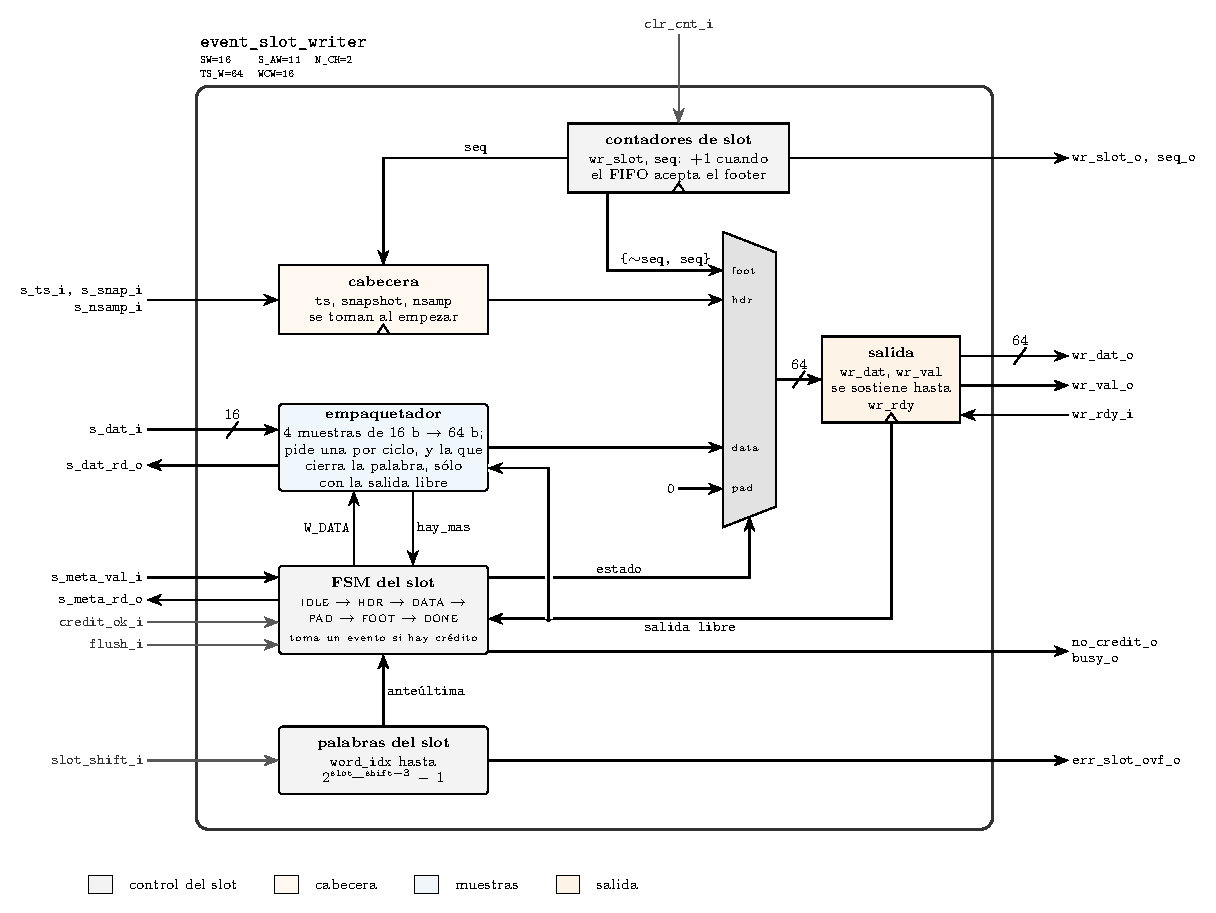
\includegraphics{cap8_panorama_slot_writer}
\caption[Vista general de \codigo{event\_slot\_writer}]{%
Vista general de \codigo{event\_slot\_writer}. El estado de la FSM elige qué
palabra sale: cuatro de cabecera, las muestras empaquetadas de a cuatro, el
relleno de ceros y el footer \codigo{\{\textasciitilde seq, seq\}}. Cada palabra
se sostiene hasta que el \codigo{axi\_wr\_fifo} la acepta, así que la
contrapresión frena al escritor sin perder muestras; \codigo{wr\_slot} y
\codigo{seq} suben recién cuando se acepta el footer.\label{f:osc-panorama-writer}}
\end{figure}

\textbf{FSM del slot}: en la Fig.~\ref{f:osc-fsm-writer} se presenta la FSM de
trabajo, que cuenta con 6 estados que forman un ciclo bajo funcionamiento
típico. El módulo de comprobación de créditos trabaja ciclo a ciclo, y se tiene
la variable \codigo{credit\_ok} en alto cuando los créditos libres son mayores a
cero.
\begin{itemize}
  \item Bajo un reset se va a \codigo{W\_IDLE}, donde espera a tener créditos de
    escritura y un evento completo en la cola de metadatos
    (\codigo{s\_meta\_val}). Con las dos condiciones copia los metadatos,
    calcula el largo del slot y pasa a \codigo{W\_HDR}. Sin créditos \textbf{no
    descarta, se frena}: la contrapresión sube al stage y el descarte ocurre
    arriba, en la captura, donde se puede descartar el evento entero y
    contarlo. \codigo{W\_DONE} da el slot por cerrado cuando el footer fue
    aceptado por el \codigo{axi\_wr\_fifo}: ahí avanzan \codigo{wr\_slot} y
    \codigo{seq}, hace el pop del metadato y vuelve a \codigo{W\_IDLE}.
\end{itemize}
En \codigo{W\_HDR}, \codigo{W\_DATA}, \codigo{W\_PAD} y \codigo{W\_FOOT} cada
palabra espera que el \codigo{axi\_wr\_fifo} la acepte (\codigo{wr\_rdy}) para
continuar con el paso. La lógica interna de la FSM se presenta en la
Fig.~\ref{f:osc-fsm-writer}.

\begin{figure}[H]
\centering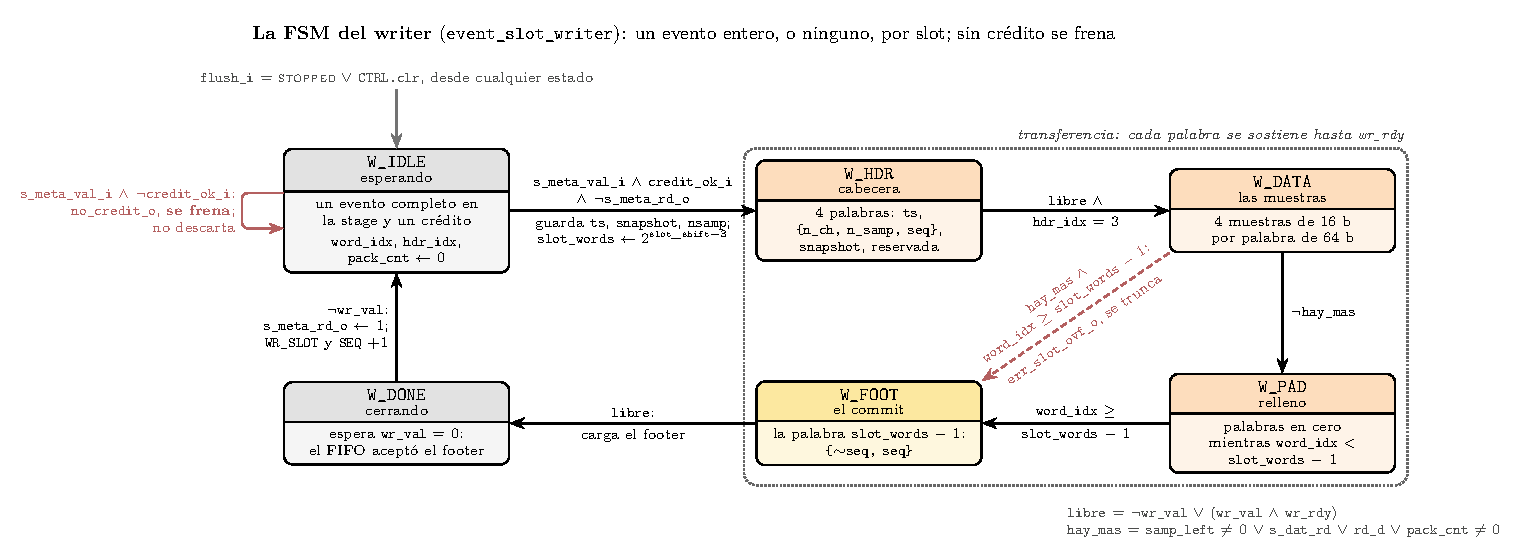
\includegraphics{cap8_fsm_slot_writer}
\caption[FSM del escritor de slots]{%
FSM del escritor de slots. Tiene tres fases: \codigo{W\_IDLE}, la transferencia
(el grupo punteado: \codigo{W\_HDR}, \codigo{W\_DATA}, \codigo{W\_PAD} y
\codigo{W\_FOOT}) y \codigo{W\_DONE}. Sin crédito se queda en \codigo{W\_IDLE}
con \codigo{no\_credit = 1}: se frena, no descarta. En la transferencia cada
palabra se sostiene hasta que el \codigo{axi\_wr\_fifo} la acepta, y el slot se
cierra recién cuando el FIFO acepta el footer.\label{f:osc-fsm-writer}}
\end{figure}

% Bibliografía de este capítulo. Va al final del archivo, siempre.
\bibliografiacapitulo

%%% Local Variables:
%%% mode: latex
%%% TeX-master: "template"
%%% End:
